% !TEX encoding = UTF-8 Unicode
% !TEX program = xelatex

\documentclass[
    11pt, % Set the default font size, options include: 8pt, 9pt, 10pt, 11pt, 12pt, 14pt, 17pt, 20pt
    aspectratio=169, % Set the aspect ratio to a 16:9 ratio which matches the aspect ratio of 1080p and 4K screens and projectors
]{beamer}
\usepackage[american, russian]{babel}
\usepackage{fontspec}
\setmainfont{Arial}
\setsansfont{Calibri}
\def\contentsname{Оглавление}%


% This template is inspired by the VT Presentation Template, as well as the THU Beamer Theme. Many thanks!

\graphicspath{{images/}{./}} % Specifies where to look for included images (trailing slash required)
\usepackage{booktabs} % Allows the use of \toprule, \midrule and \bottomrule for better rules in tables
%\usepackage{calligra} % Font for wordart
% \usepackage{appendixnumberbeamer} % If you want a separate slide counter for your appendix
\usepackage{fnpct} % Eliminate the unwanted space before the footnote mark
\usepackage{listings} % For code display
\usepackage{physics}

%---------------------------------------------------------
%	FOOTNOTES & CITATIONS BASIC SETUP
%---------------------------------------------------------
% Check FOOTNOTES & CITATIONS ADVANCED SETUP for solutions for intra- and inter-frame citations
% The workarounds in ADVANCED SETUP require the style to be "numeric"
% If you're good without ADVANCED SETUP, comment out the ADVANCED SETUP section, and pick whatever style you like
% \usepackage[style=authoryear, backend=bibtex]{biblatex}
\usepackage[style=numeric, sorting=none, backend=biber]{biblatex}
\addbibresource{bib.bib}
\setbeamerfont{footnote}{size=\tiny}
% The lines below set the citation style to "number, title, year". The ADVANCED SETUP will overwrite this style
\usepackage{xpatch}
\xapptobibmacro{cite}{\setunit{\nametitledelim} \printfield{title} \setunit{\nametitledelim} \printfield{year}}

%---------------------------------------------------------
%	FOOTNOTES & CITATIONS ADVANCED SETUP
%---------------------------------------------------------
% Manage faulty intra- and inter-frame footnotes and citations. References:
%     https://tex.stackexchange.com/a/520777
%     https://topanswers.xyz/tex?q=453

% You might want to use \firstcite and \secondcite instead of \footnote in your document
% Mark the first citation with \firstcite and the rest with \secondcite

% \renewcommand{\thefootnote}{\arabic{footnote}} % Switch to footnote with numbers
% \renewcommand{\thefootnote}{\alph{footnote}} % Switch to footnote with letters

\DeclareCiteCommand{\firstcite}
{\usebibmacro{prenote}}
{%
    \footnotemark[\thefield{labelnumber}]% mark corresponding to the number entry
    \footnotetext[\thefield{labelnumber}]{% footnote text corresponding to the number entry
        \printnames{labelname}% name
        \setunit{\printdelim{nametitledelim}}% separator
        % \setunit{\addperiod\space}% another way to add separator
        \printfield[citetitle]{labeltitle}% title
        \setunit{\printdelim{nametitledelim}}% separator
        \printfield{year}% year
        \newunit{\adddot}% ending dot
    }%
}
{\multicitedelim}
{\usebibmacro{postnote}}

\DeclareCiteCommand{\secondcite}
{\usebibmacro{prenote}}
{%
    \footnotemark[\thefield{labelnumber}]% mark corresponding to the number entry
}
{\multicitedelim}
{\usebibmacro{postnote}}

%---------------------------------------------------------
%	SELECT THEME & COLORS
%---------------------------------------------------------
\usetheme{Madrid} % You can use other themes too, but this changes many things. I've found Madrid to be the best for this color scheme

% fg = foreground color
% bg = background color

% Many colors are linked to multiple attributes, change with caution!
\definecolor{smuBlue}{RGB}{0,86,145}
%\definecolor{smuGold}{RGB}{138, 112, 76}
\definecolor{scisGold}{RGB}{255, 140, 0}

\setbeamercolor*{structure}{bg=smuBlue, fg=smuBlue}
% Title block and bottom right box color
\setbeamercolor*{palette primary}{use=structure, fg=white,bg=smuBlue} % Bottom left box and bar between title & top bubbles
\setbeamercolor*{palette secondary}{use=structure, fg=smuBlue, bg=white}
% Probably not used
\setbeamercolor*{palette tertiary}{use=structure, fg=white, bg=smuBlue} 

% Title of each slide
\setbeamercolor{frametitle}{bg=smuBlue, fg=white}
\setbeamercolor*{titlelike}{parent=palette primary}

%%% Headline and Central Footer %%%
% You can change the theme back and forth for each frame
% Theme I - white head, white foot
    % \setbeamercolor{section in head/foot}{fg=scisGold, bg=white}
    % \setbeamercolor{headline}{fg=scisGold, bg=white}
% Theme II - gold head, gold foot (as shown in the title frame)
    \setbeamercolor{section in head/foot}{fg=black, bg=scisGold}
    \setbeamercolor{headline}{fg=white, bg=scisGold}
% Theme III - white head, gold foot (as shown in the rest of the frames)
    % \setbeamercolor{section in head/foot}{fg=scisGold, bg=white}
    % \setbeamercolor{title in head/foot}{fg=white, bg=scisGold}
    % \setbeamercolor{headline}{fg=scisGold, bg=white}

%%% Specific Colors %%%
\setbeamercolor{item projected}{bg=scisGold}
\setbeamertemplate{enumerate items}{bg=scisGold}

\setbeamercolor{itemize item}{fg=scisGold}
\setbeamercolor{itemize subitem}{fg=scisGold}

\setbeamercolor{button}{bg=scisGold}

%%% Edits ONLY the TOC slide %%%
\setbeamercolor{section in toc}{fg=black}
\setbeamercolor{subsection in toc}{fg=black}

%%% Block Colors %%%
% Standard block
    \setbeamercolor{block title}{bg=scisGold, fg=white}
    \setbeamercolor{block body}{bg=scisGold!20}
% Alerted block
    \setbeamercolor{block title alerted}{bg=orange, fg=white}
    \setbeamercolor{block body alerted}{bg=orange!10}
% Example block
    \setbeamercolor{block title example}{bg=smuBlue, fg=white}
    \setbeamercolor{block body example}{bg=smuBlue!10}

%---------------------------------------------------------
%	SELECT THE FONT THEME & FONTS
%---------------------------------------------------------
\usefonttheme{default} % Typeset using the default sans serif font
%\usepackage{palatino} % Use the Palatino font for serif text
%\usepackage[default]{opensans} % Use the Open Sans font for sans serif text
\useinnertheme{circles}

%---------------------------------------------------------
%	SELECT THE OUTER THEME
%---------------------------------------------------------
% Outer themes change the overall layout of slides, such as header and footer lines, sidebars and slide titles. Uncomment each theme in turns to see what changes it makes to your presentation.

%\useoutertheme{default}
\useoutertheme{miniframes}
%\usepackage{ulem}
%\useoutertheme{infolines}
 %\useoutertheme{smoothbars}
 %\useoutertheme{sidebar}
 %\useoutertheme{split}
 %\useoutertheme{shadow}
 %\useoutertheme{tree}
 %\useoutertheme{smoothtree}
 \usepackage{adjustbox}
 \usepackage{multicol}

%---------------------------------------------------------
%	PRESENTATION INFORMATION
%---------------------------------------------------------
\title{Исследование динамики поляризованного пучка в
	ускорительном комплексе NICA-Nuclotron в приложении
	к изучению электрического дипольного момента легких
	ядер}
\subtitle{Специальность 1.3.2 «Приборы и методы экспериментальной физики»}
\author{Соискатель к.ф.-м.н.: Колокольчиков C. Д.}

\institute[]{
{\normalsize Научный руководитель: профессор, д.ф.-м.н. Сеничев Ю.В.}\newline \newline
Институт Ядерных Исследований РАН, Москва, Россия}
\date[29 сентября 2025]
% \date[\today]

% School logo
% You can enable and disable logo display for each frame
\logo{
\includegraphics[width=1cm]{logo.eps}}

%---------------------------------------------------------
%	CODE DISPLAY
%---------------------------------------------------------
\lstset{
    basicstyle=\ttfamily\small,
    keywordstyle=\bfseries\color{blue},
    emphstyle=\ttfamily\color{red},   
    stringstyle=\color{green},
    numbers=left,
    numberstyle=\small\color{gray},
    rulesepcolor=\color{red!20!green!20!blue!20},
    frame=shadowbox,
    xleftmargin=1cm,
    xrightmargin=1cm,
}

%---------------------------------------------------------
%	EXTRA SETTINGS
%---------------------------------------------------------

% Clear warnings related to \translate
%     https://github.com/josephwright/beamer/issues/449
\pdfstringdefDisableCommands{
    \def\translate#1{#1}
}

% Adjust header height
\setbeamertemplate{headline}{
    \nointerlineskip
    \begin{beamercolorbox}[wd=\paperwidth,ht=7.0ex]{headline}
        \insertnavigation{\paperwidth}\vspace*{2.0ex}
    \end{beamercolorbox}
}

% Disable navigation symbols
\setbeamertemplate{navigation symbols}{}

%---------------------------------------------------------
%   DOCUMENT BEGINS
%---------------------------------------------------------
\begin{document}

%---------------------------------------------------------
%	TITLE SLIDE
%---------------------------------------------------------
\section{}

% Set background
\usebackgroundtemplate{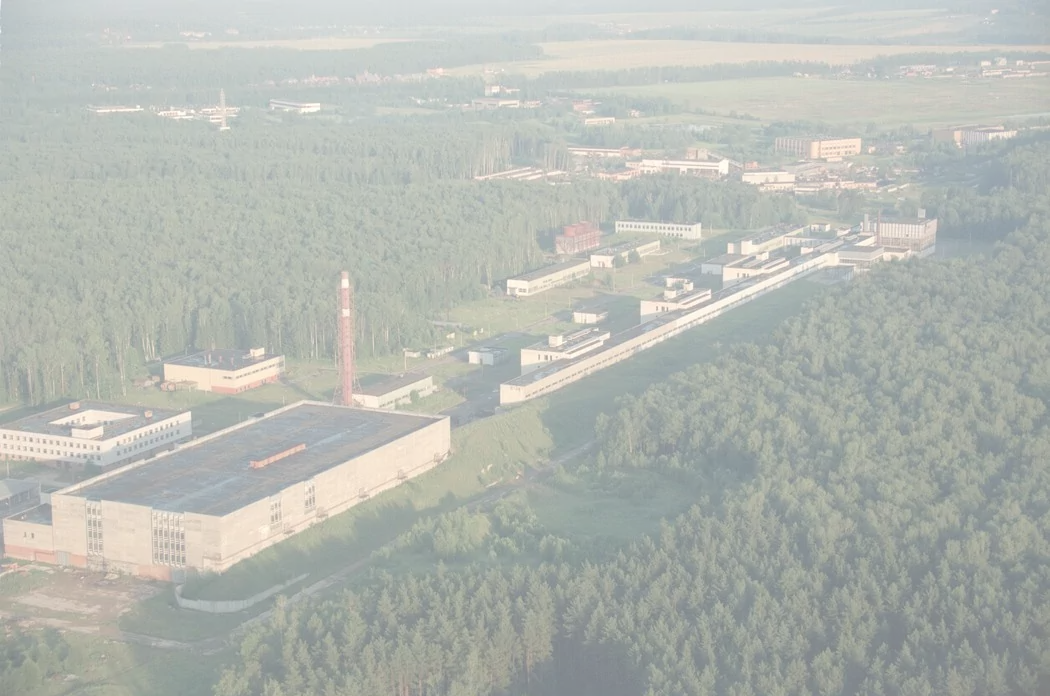
\includegraphics[width=\paperwidth]{meson_title.png}}


% Disable logo
\logo{}

\begin{frame}
	\titlepage % Output the title slide, automatically created using the text entered in the PRESENTATION INFORMATION block above
\end{frame}

% Clear background
\usebackgroundtemplate{}
% Enable logo
\logo{
\includegraphics[width=1cm]{logo.eps}}

% Switch to Theme III
%\setbeamercolor{section in head/foot}{fg=scisGold, bg=white}
%\setbeamercolor{title in head/foot}{fg=white, bg=scisGold}
%\setbeamercolor{headline}{fg=scisGold, bg=white} 

%%---------------------------------------------------------
%	TABLE OF CONTENTS SLIDE
%---------------------------------------------------------
% References sections and subsections, specified with the standard \section and \subsection commands. If you want to display all sections and subsections on one slide, just use \tableofcontents. If you want to just display each section one at a time (in subsequent slides) use \tableofcontents[pausesections].

\begin{frame}
	\frametitle{Оглавление} % Slide title, remove this command for no title
	\tableofcontents % Output the table of contents (all sections on one slide)
	%\tableofcontents[pausesections] % Output the table of contents (break sections up across separate slides)
\end{frame}
%------------------------------------------------
\section{Введение}
%------------------------------------------------
\begin{frame}
 \frametitle{Актуальность}
 	\begin{itemize}
 		\item Исследование кварк-глюонной плазмы;
 		\item Разрешение проблемы "спинового кризиса";
 		\item Изучение Электрического Дипольного Момента;
 		\item Поиск аксионоподобных частиц.
 	\end{itemize}

	 %\begin{figure}
	 %	\centering
	 %	\includegraphics[width=0.24\linewidth]{"images/EDM CP"}
	 %	\includegraphics[width=0.74\linewidth]{"images/EDM World"}
	 %\end{figure}

\end{frame}
%------------------------------------------------
\begin{frame}
	\frametitle{Цель и Задачи исследования}
	\textbf{Целью} данной диссертации является изучение особенностей поведения лёгких поляризованных пучков в предлагаемой дуальной структуре, а также исследования ЭДМ с использованием квази-замороженной концепции.\newline \newline
	Для достижения поставленной цели необходимо было решить следующие \textbf{задачи}:
	\begin{itemize}
		\item Определение требований к дуальной структуре для тяжелых ионов;
		\item Регулирование критической энергии для поляризованных частиц методом резонансной модуляции дисперсионной функции;
		\item Проведение численного моделирования продольной динамики частиц;
		\item Изучение концепции «квази-замороженного» спина с целью создания установки для исследования ЭДМ дейтрона и протона;
	\end{itemize}
\end{frame}
%------------------------------------------------
\begin{frame}
	\frametitle{Научная новизна}
	\begin{itemize}
		\item	Впервые предложена дуальная структура для тяжелых ионов и легких частиц для коллайдера NICA;
		\vspace{1em}
		\item 	Впервые предложены методы подавления дисперсии поворотной аркой в резонансной магнитооптической структуре с отсутствующими магнитами;
		\vspace{1em}
		\item	Впервые исследован метод скачка критической энергии с использованием барьерного ускоряющего потенциала с учётом ограничений по продольной микроволновой неустойчивости;
	\end{itemize}
	
\end{frame}
%------------------------------------------------
\begin{frame}
	\frametitle{Научная новизна}
	\begin{itemize}
		\item 	Были проведены исследования продольной динамики с учётом высших порядков разложения по импульсу, а также влиянием импеданса. На их базе сформулированы ограничения на величину и темп скачка критической энергии;
		\vspace{1em}
		\item	Были разработаны 8- и 16-периодичная квази-замороженная структура Nuclotron для выделения ЭДМ сигнала лёгких ядер;
		\vspace{1em}
		\item	Была разработана структура коллайдера NICA с обводными каналами, неориентированная изначально на эксперименты по поиску ЭДМ дейтрона методом квази-замороженного спина;
	\end{itemize}
\end{frame}
%------------------------------------------------
\begin{frame}
	\frametitle{Практическая значимость}
	Исследования направлены на формирование полноценной физической программы в комплексе Nuclotron-NICA. \\
	Применение изложенных в работе подходов возможно и на других похожих установках без потери общности.
\end{frame}
%------------------------------------------------
\begin{frame}
	\frametitle{Объект исследования}
	% TODO: \usepackage{graphicx} required
	\begin{figure}
		\centering
		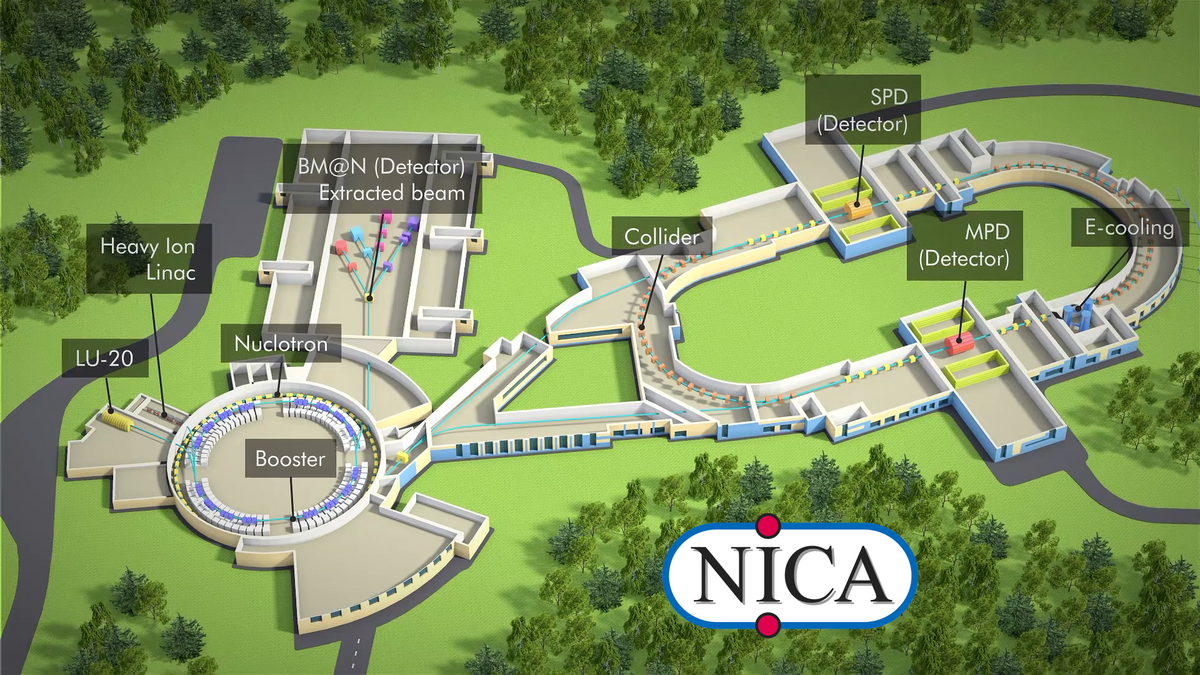
\includegraphics[width=0.6\linewidth]{images/NICA}
	\end{figure}
	В работе отдается приоритет исследованиям свойств пучков частиц, где ускоритель выступает в роли детектирующего устройства.
\end{frame}
%------------------------------------------------
\begin{frame}
	\frametitle{Методы исследования}
	\begin{enumerate}
		\item	Аналитические и численные;
		\item	Экспериментальные;
	\end{enumerate}
	\vspace{2em}
	\textbf{Математическое и компьютерное моделирование}. Были использованы программы для расчёта поперечной динамики: MAD-X, OPTIM, BMAD, продольной динамики: BLonD; спин-орбитальной динамики: COSY Infinity.\\
	\vspace{1em}
	\textbf{Экспериментальные} методы исследования заключаются в изучении динамики пучка с применением скачка критической энергии и без него.
	Соискатель лично участвовал в сеансе на синхротроне У-70 в г. Протвино, Россия в 2023 году.

\end{frame}
%------------------------------------------------
\begin{frame}
	\frametitle{Основные положения, выносимые на защиту}
	\begin{itemize}
		\item 	Предложена реализация дуальной структуры для комплекса NICA-Nuclotron, оптимальная для тяжелых ионов с точки зрения ВПР и лёгких частиц с поднятой критической энергией;
		\vspace{1em}
		\item	Реализован метод вариации критической энергии для коллайдера NICA с отсутствующими магнитами при подавлении дисперсионной функции двумя семействами квадруполей и двумя крайними ячейками;
		\vspace{1em}
		\item	Представлены результаты моделирования продольной динамики с учётом высших порядков разброса по импульсам и моделей продольных импедансов в окрестности критической энергии и сравнение с экспериментальными данными на У-70;
	\end{itemize}
\end{frame}
%------------------------------------------------
\begin{frame}
	\frametitle{Основные положения, выносимые на защиту}
	\begin{itemize}
		\item	Проведен анализ использования гармонического ВЧ при процедуре скачка в коллайдере NICA. Для барьерного ВЧ представлены данные моделирования продольной динамики. Предложено сокращение длины между барьерами из-за продольной микроволновой неустойчивости;
		\vspace{1em}
		\item	Предложены модернизированные 8/16-периодичные структуры Nuclotron с квази-замороженным спином для исследования ЭДМ лёгких ядер, с сохранением функции бустера;
		\vspace{1em}
		\item	Применен метод фильтров Вина для сохранении направления поляризации на основе введения обводных каналов в структуре коллайдера NICA с квази-замороженным спином;
	\end{itemize}
\end{frame}
%------------------------------------------------
%------------------------FIRST------------------------
%------------------------------------------------

\begin{frame}
	\frametitle{Содержание доклада}
	\begin{enumerate}
	\item Дуальная структура;\newline
	\item Прохождение критической энергии;\newline
	\item Исследование ЭДМ.
	\end{enumerate}
\end{frame}
%------------------------------------------------
\section{Дуальная структура}
%------------------------------------------------
\begin{frame}
	\centering \Large{Дуальная структура}
\end{frame}
%------------------------------------------------
\begin{frame}
	\frametitle{Дуальная структура}
	При разработке структуры, удовлетворяющей требованиям, предъявляемым к частицам с различным зарядом, важно создать перестраиваемую структуру без внесения конструктивных изменений. Мы назвали такую структуру -- \textit{дуальной}.
	\vspace{2em} 
	
	\begin{columns}
		\begin{column}{0.5\textwidth}
			\raggedright
			\adjustbox{valign=t}{\begin{minipage}[t]{\linewidth}
				\centering \textbf{Тяжёлые ионы}\\
				обладают более выраженным эффектом разогрева из-за внутрипучкового рассеяния.\\
			\end{minipage}}
		\end{column}
		\hfill
		\begin{column}{0.5\textwidth}
			\raggedright
			\adjustbox{valign=t}{\begin{minipage}[t]{\linewidth}
				\centering{\textbf{Лёгкие частицы}}\\
				влияние критической энергии на динамику сгустка.\\
			\end{minipage}}
		\end{column}
		\begin{column}{0.01\textwidth}
		\end{column}
	\end{columns}
	\vspace{2em}
\footnotetext[1]{(to be published) Kolokolchikov S.D., et al. Features of dual-purpose structure for heavy ion and light particles, Nucl.Sci. and Tech.}		
\end{frame}
%------------------------------------------------
\begin{frame}
	\frametitle{Регулярная структура}
	\begin{columns}
		\begin{column}{0.3\textwidth}
			\raggedright
			\adjustbox{valign=t}{\begin{minipage}[t]{\linewidth}
				В классической регулярной структуре $\gamma_{\text{tr}}\simeq\nu_{x}$. \\
				При одинаковой магнитной жесткости $B\rho$ максимальная энергия для легких частиц выше, чем для тяжелых ионов, из-за их соотношения заряд-масса.
			\end{minipage}}
		\end{column}
		\begin{column}{0.7\textwidth}
			\begin{minipage}{\linewidth}
				\centering
				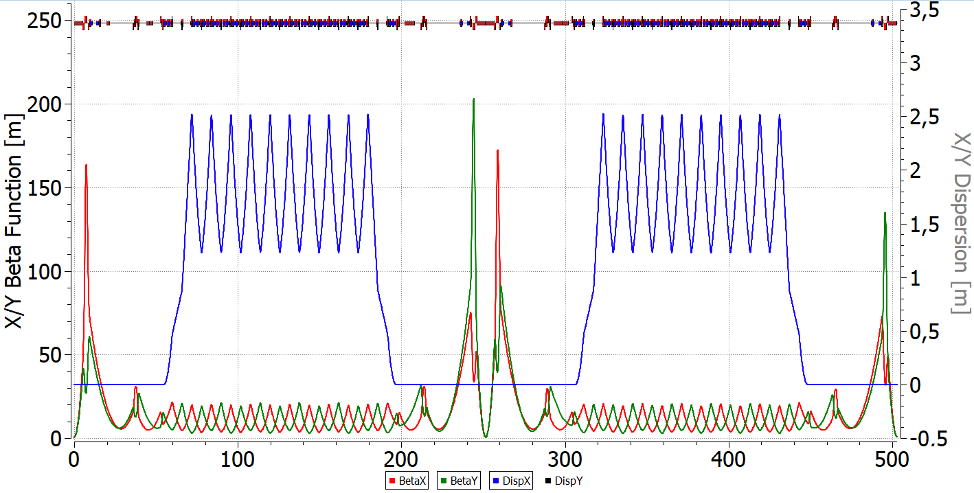
\includegraphics[width=1\linewidth]{images/1_regular}
			\end{minipage}
		\end{column}
	\end{columns}
\end{frame}
%------------------------------------------------
\begin{frame}
	\frametitle{Резонансная структура}
	\begin{columns}
	\begin{column}{0.3\textwidth}
		\raggedright
		\adjustbox{valign=t}{\begin{minipage}[t]{\linewidth}
		Может быть получена из регулярной структуры путем разделения фокусирующих квадруполей на 2 семейства с различными градиентами.		
		\end{minipage}}
	\end{column}
	\begin{column}{0.7\textwidth}
		\begin{minipage}{\linewidth}
			\centering
			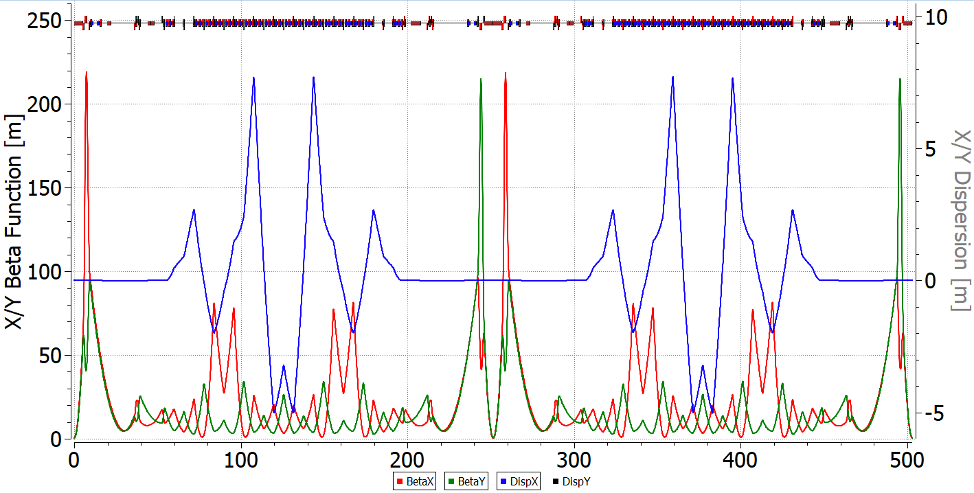
\includegraphics[width=1\linewidth]{images/1_resonant}
		\end{minipage}
	\end{column}
\end{columns}
\footnotetext[2]{Колокольчиков С.Д., Сеничев Ю.В. Магнито-оптическая Структура Коллайдера NICA c Высокой Критической Энергией. Яд. Физ. и Инж. том 13, номер 1, стр. 27-36 (2022). DOI: 10.56304/S2079562922010171}
\footnotetext[3]{Колокольчиков С.Д., Сеничев Ю.В. Особенности Прохождения и Повышения Критической Энергии Синхротрона. Яд. Физ. и Инж. том 14, номер 6, стр. 587-592 (2023).  DOI: 10.56304/S2079562923010153}
\end{frame}
%------------------------------------------------
\begin{frame}
	\frametitle{Комбинированная структура}
	\begin{columns}
		\begin{column}{0.3\textwidth}
			\raggedright
			\adjustbox{valign=t}{\begin{minipage}[t]{\linewidth}
					Реальная арка
					\begin{equation} \label{eq:eta_pk}
						\eta_{\textrm{pk}}=\frac{1}{\gamma_{\textrm{tr}}^2}-\frac{1}{\gamma^2}
					\end{equation}
					\noindent компенсируется аркой с комплексным значением критической энергии
					\begin{equation} \label{eq:eta_kp}
						\eta_{\textrm{kp}}=-\frac{1}{\gamma_{\textrm{tr}}^2}-\frac{1}{\gamma^2}\ \ \ 
					\end{equation}
			\end{minipage}}
		\end{column}
		\begin{column}{0.7\textwidth}
			\begin{minipage}{\linewidth}
				\centering
				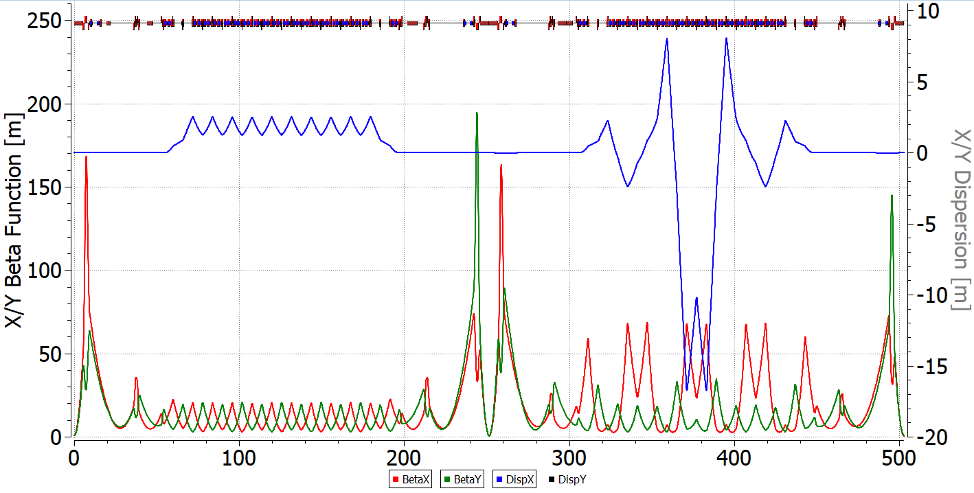
\includegraphics[width=1\linewidth]{images/1_combined}
			\end{minipage}
		\end{column}
	\end{columns}
\end{frame}
%------------------------------------------------
\begin{frame}
	\frametitle{Стохастическое охлаждение}
	\begin{equation}
		\frac{1}{\tau_{\text{tr,l}}}=A\cdot\frac{W}{N} \frac{\left(1-1 / {M_{\text{pk}}}^2\right)^2}{M_{\text{kp}}}; \quad
		M_{\text{pk}} =\frac{1}{2\left(f_{\max}+f_{\min}\right) \eta_{\textrm{pk}} T_{\textrm{pk}} \delta}; \quad 
		M_{\text{kp}} =\frac{1}{2\left(f_{\max}-f_{\min}\right) \eta_{\textrm{kp}} T_{\textrm{kp}} \delta}.
	\end{equation}

	\begin{columns}
		\begin{column}{0.5\textwidth}
			\raggedright
			\adjustbox{valign=t}{\begin{minipage}[t]{\linewidth}
				Асимптотический рост в двух случаях:
				\begin{enumerate}
					\item $\eta\rightarrow\frac{1}{2\left(f_{\text{max}}+f_{\text{min}}\right)T_{\text{pk}}\delta}$, Schottky-спектр пучка становится сплошным и $M_{\text{pk}}\rightarrow1$;
					\item $\eta\rightarrow0$, перемешивание на пути от киккера к пикапу не происходит и $M_{\text{kp}}\rightarrow\infty$.
				\end{enumerate}
			\end{minipage}}
		\end{column}
		\begin{column}{0.5\textwidth}
			\begin{minipage}{\linewidth}
				\centering
				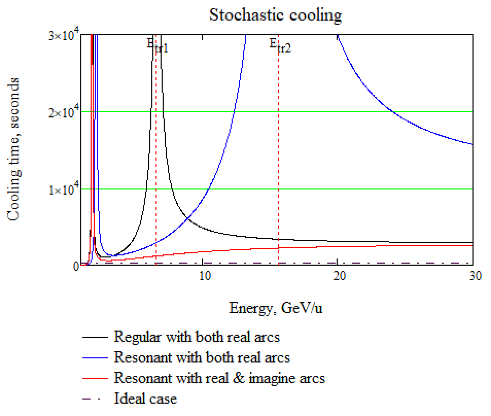
\includegraphics[width=0.7\linewidth]{images/1_SC_wide}
			\end{minipage}
		\end{column}
	\end{columns}
\end{frame}
%------------------------------------------------
\begin{frame}
	\frametitle{Внутрипучковое рассеяние}
	\begin{equation}
		\frac{1}{\tau_x}=\frac{\pi^2r_0^2v_cm^3N\left(log\right)}{\gamma\Gamma}\left[\frac{\gamma^2\left(D_x^2+\beta_x^2\phi_x^2\right)}{\epsilon_x\beta_x}\right]\int_{0}^{\infty}\frac{d\lambda\ \lambda^\frac{1}{2}\left[a_x\lambda+b_x\right]}{\left(\lambda^3+a\lambda^2+b\lambda+c\right)^\frac{3}{2}}
		\label{eq:IBS}
	\end{equation}
	
	\begin{columns}
		\begin{column}{0.4\textwidth}
			\raggedright
			\adjustbox{valign=t}{\begin{minipage}[t]{\linewidth}
					Из сравнения времени внутрипучкового рассеяния со временем охлаждения можно сделать заключение, что в регулярной структуре стохастическое охлаждение способно сбалансировать внутрипучковое рассеяние в диапазоне энергий $W\geq4.5$ ГэВ/нуклон.
			\end{minipage}}
		\end{column}
		\begin{column}{0.6\textwidth}
			\begin{minipage}{\linewidth}
				\centering
				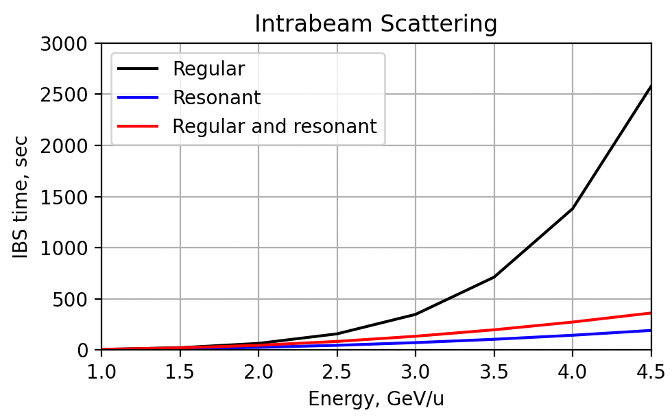
\includegraphics[width=0.8\linewidth]{images/1_IBS}
			\end{minipage}
		\end{column}
	\end{columns}
\end{frame}
%------------------------------------------------
%------------------------SECOND------------------------
%------------------------------------------------
\section{Прохождение критической энергии}
%------------------------------------------------
\begin{frame}
	\centering \Large{Прохождение критической энергии}
\end{frame}
%------------------------------------------------
\begin{frame}
	\frametitle{Скачок критической энергии в У-70}
	
	\begin{columns}
		\begin{column}{0.4\textwidth}
			\raggedright
			\adjustbox{valign=t}{\begin{minipage}[t]{\linewidth}
				Вспомогательные квадруполи расположены через полпериода $\Delta\nu_{x,y}=0.5\times0.5$ и имеют противоположные полярности.
				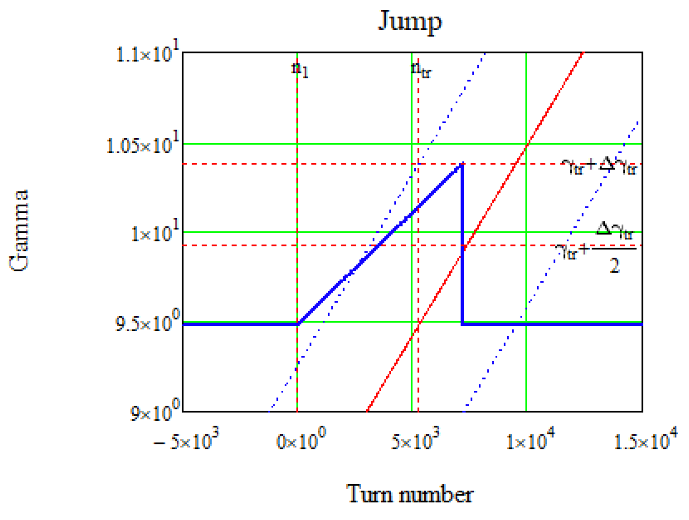
\includegraphics[width=1\columnwidth]{images/3_gamma_transition_jump_U70.png}
			\end{minipage}}
		\end{column}
		\begin{column}{0.4\textwidth}
			\begin{minipage}{\linewidth}
				\centering
				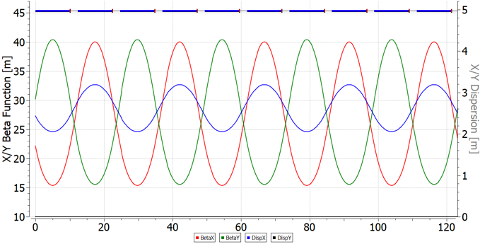
\includegraphics[width=1\columnwidth]{images/3_twiss_U70_regular.png}
				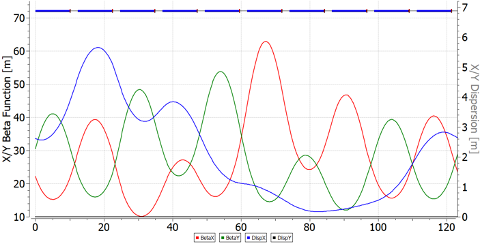
\includegraphics[width=1\columnwidth]{images/3_twiss_U70_modulated.png}
			\end{minipage}
		\end{column}
	\end{columns}
\end{frame}
%------------------------------------------------
\begin{frame}
	\frametitle{Данные с сеанса на У-70}
	\centering
	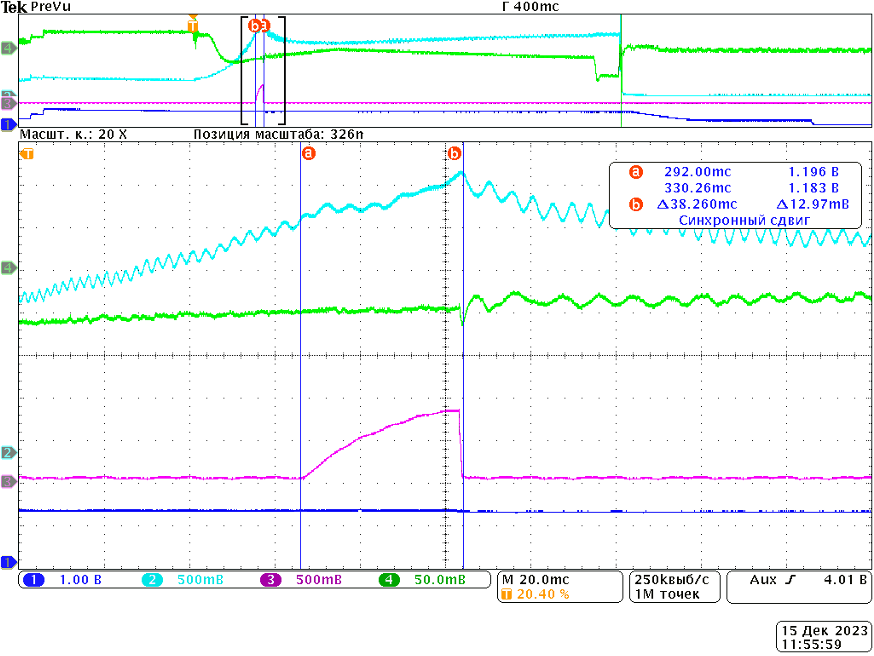
\includegraphics[width=0.30\columnwidth]{3_jump_U70_oscilogram.png}
	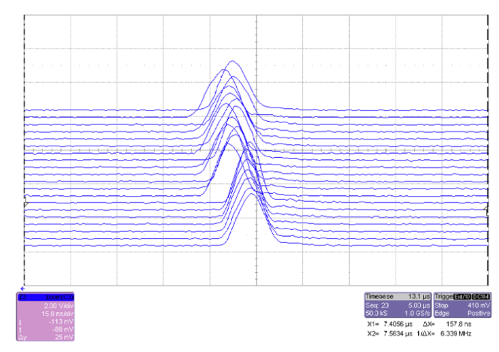
\includegraphics[width=0.323\columnwidth]{3_jump_U70_beam_profile.png}
	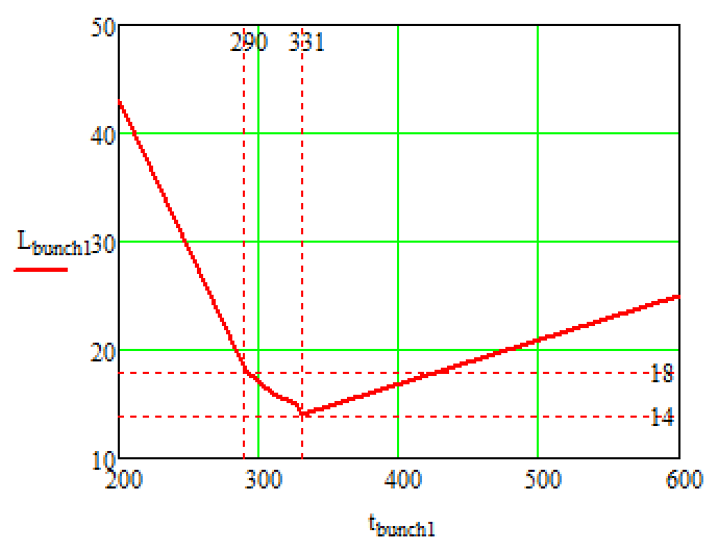
\includegraphics[width=0.30\columnwidth]{3_jump_U70_beam_lenght.png}
\footnotetext[4]{Kolokolchikov, S.D., Senichev, Y.V. \& Kalinin, V.A. Transition Energy Crossing in Harmonic RF at Proton Synchrotron U-70. Phys. Atom. Nuclei 87, 1355–1362 (2024). https://doi.org/10.1134/S106377882410020X}
\end{frame}
%------------------------------------------------
\begin{frame}
	\frametitle{Скачок критической энергии в NICA}
	
	Для NICA $\Delta\gamma_{\textrm{tr}}=1.1\Delta q$. Максимальная вариация частоты или рабочей точки составляет $\pm\Delta q=0.05$, что соответствует измерению критической энергии порядка $\Delta\gamma_{\textrm{tr}}=0.09$
	
	\centering
	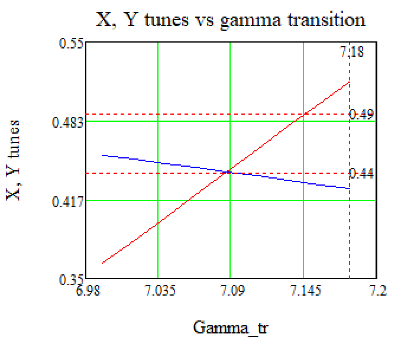
\includegraphics[width=0.35\columnwidth]{3_tunes_vs_g_tr.png}
	\includegraphics[width=0.35\linewidth]{3_Jump_NICA}
\footnotetext[5]{Kolokolchikov S.D. et al. Transition Energy Crossing in NICA Collider of Polarized Proton Beam in Harmonic and Barrier RF. Phys. Atom. Nuclei 87, 1449–1454 (2024). DOI: 10.1134/S1063778824100211}
\end{frame}
%------------------------------------------------
\begin{frame}
	\frametitle{Скачок критической энергии в барьерном ВЧ}
	\centering
	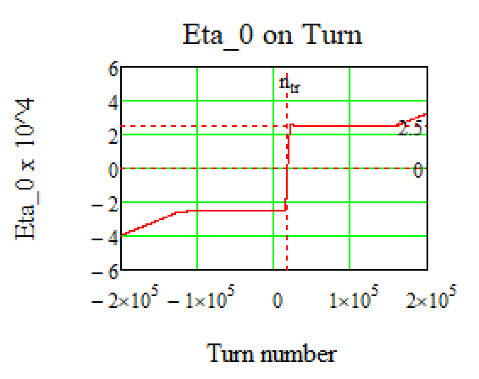
\includegraphics[width=0.4\columnwidth]{3_eta_tr_BB.png}
	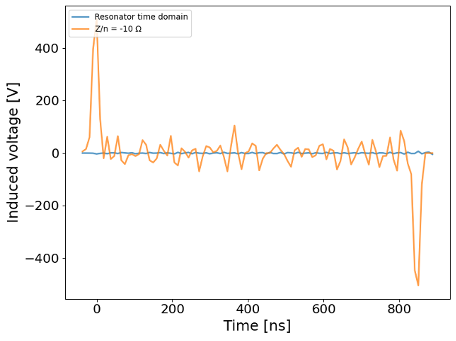
\includegraphics[width=.45\columnwidth]{3_induced_voltage}
\footnotetext[6]{Kolokolchikov S. et al. Longitudinal Dynamic in NICA Barrier Bucket RF System at Transition Energy Including Impedances in BLonD. Phys. Part. Nuclei Lett. 21, 419–424 (2024). DOI: 10.1134/S1547477124700389}
\footnotetext[7] {Kolokolchikov S., Acceleration and crossing of transition energy investigation using an RF structure of the barrier bucket type in the NICA accelerator complex. J.Phys.Conf.Ser. Vol. 2420, 012001 (2023). DOI: 10.1088/1742-6596/2420/1/012001}
\end{frame}
%------------------------------------------------
\begin{frame}
	\frametitle{Продольная микроволновая неустойчивость}
	\begin{equation}
		N_p\le K_1K_2\frac{E_0}{\left(\left|Z_\parallel\right|/n\right)ec}\left|\eta\right|\gamma\beta\sigma_p^2L_{\textrm{B}};
		\quad \quad
		N_p\le K_1K_2\frac{E_0}{\left(\left|Z_\parallel\right|/n\right)ec}\left|\eta\right|\frac{4\varepsilon_{\text{tr}}^2}{{\pi\gamma\beta L}_{\textrm{B}}}
		\label{eq:microwave_instability_2}
	\end{equation}
	\centering
	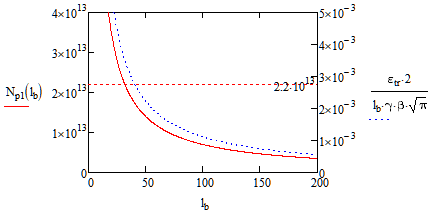
\includegraphics[width=0.6\columnwidth]{3_microwave_inst_vs_lenght.png}
\end{frame}
%------------------------------------------------
%------------------------THIRD------------------------
%------------------------------------------------
\section{Исследование ЭДМ}
%------------------------------------------------
\begin{frame}
	\centering \Large{Исследование ЭДМ}
\end{frame}
%------------------------------------------------
\begin{frame}
	\frametitle{Т-БМТ уравнение эволюции спина}
	\par В случае измерения ЭДМ заряженных частиц необходимо использование ускорителя заряженных частиц
	\par Т-БМТ уравнение описывает эволюцию поведения спина во внешних полях
	
	\begin{equation}	
		\begin{aligned} 
			\dv{{\vec{S}}}{t} &=\left(\vec{\Omega}_{\textrm{MDM}}+\vec{\Omega}_{\textrm{EDM}}\right) \times \vec{S}, \\
			\vec{\Omega}_{\textrm{MDM}}&=-\frac{q}{m \gamma}\left\{(\gamma G+1)\vec{B}_{\perp}+(G+1)\vec{B}_{\parallel}-\left(\gamma G+\frac{\gamma}{\gamma+1}\right) \frac{\vec{\beta} \times \vec{E}}{c}\right\}, \\
			\vec{\Omega}_{\textrm{EDM}}&=-\frac{q \eta}{2 m}\left(\vec{\beta} \times \vec{B}+\frac{\vec{E}}{c}-\frac{\gamma}{\gamma+1}\frac{\vec{\beta}}{c}\left(\vec{\beta}\cdot\vec{E}\right)\right), \quad G=\frac{g-2}{2}
		\end{aligned}
		\label{eq:T-BMT}
	\end{equation}
\end{frame}
%------------------------------------------------
\begin{frame}
	\frametitle{Квази-замороженный спин}
	Условия квази-замороженного спина
	\begin{equation}
		\tiny
		\Phi_p^{\textrm{arc}}+\Phi_{p}^{\textrm{comp}}=\frac{2\pi}{N};\quad \Phi_s^{\textrm{arc}}+\Phi_{s}^{\textrm{comp}}=0
		\label{eq:QFS_orbital}
	\end{equation}
	\normalsize
	Длина компенсирующего элемента
	\begin{equation}
		\tiny
		L_{\text{min}} = \Phi_{p\mathrm{E}}^{\text{comp}}R_{\mathrm{E}}=
		\frac{2\pi}{N}\frac{\gamma^2 G}{G+1}\frac{\kappa}{\mathrm{E}_{\text{max}}}
		= \frac{2\pi}{N}\frac{G}{G+1}\frac{mc^2}{e}\frac{\gamma(\gamma^2-1)}{\mathrm{E}_{\text{max}}}.
		\label{eq:length_min}
	\end{equation}
	\normalsize
	\centering
	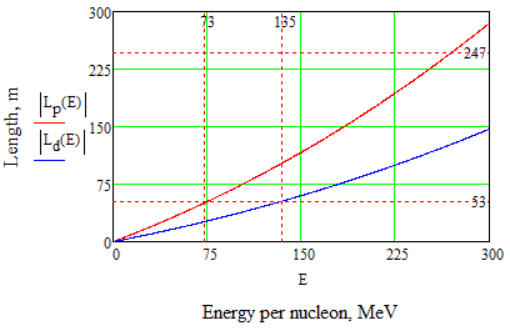
\includegraphics[width=0.3\columnwidth]{4_total_length}
\footnotetext[9]{(to be published) Kolokolchikov S.D., et al. Quasi-frozen spin for both deuteron and proton beam at periodic EDM storage ring lattice, Nucl.Sci. and Tech.}
\end{frame}
%------------------------------------------------
\begin{frame}
	\frametitle{Электростатический дефлектор}
	\centering
	а. Дейтрон\quad\quad\quad\quad\quad\quad\quad\quad\quad\quad\quad\quad\quad\quad\quad б. Протон \\
	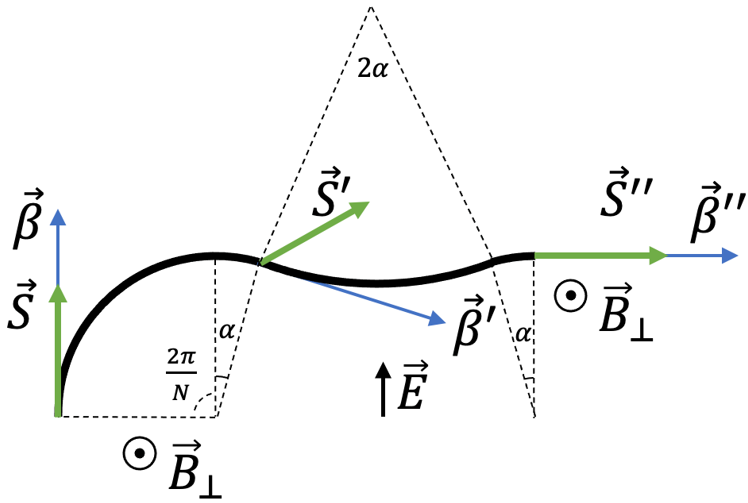
\includegraphics[width=0.4\columnwidth]{4_deflector_deutron}
	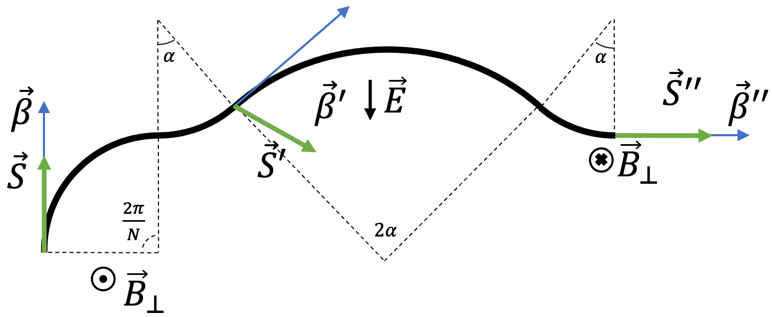
\includegraphics[width=0.5\linewidth]{4_deflector_proton}
\end{frame}
%------------------------------------------------
%------------------------------------------------
\begin{frame}
	\frametitle{Фильтр Вина}
	\centering
	а. Дейтрон\quad\quad\quad\quad\quad\quad\quad\quad\quad\quad\quad\quad\quad\quad\quad\quad б. Протон \\
	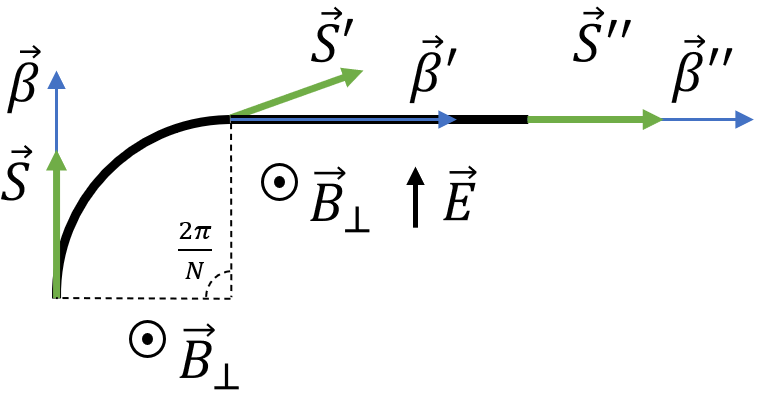
\includegraphics[width=0.49\linewidth]{4_wien-filter_deuteron}
	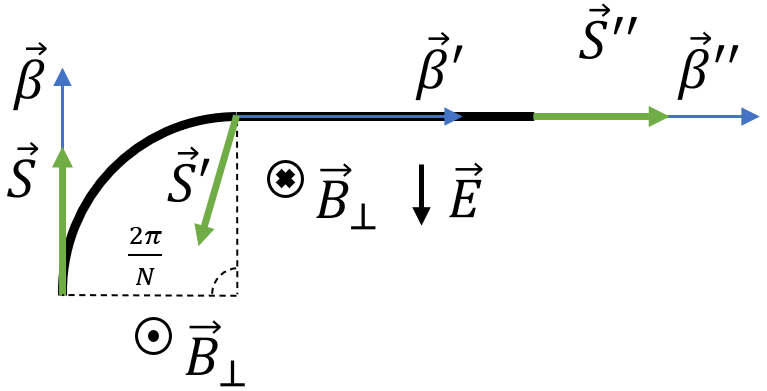
\includegraphics[width=0.49\linewidth]{4_wien-filter_proton}
\end{frame}
%------------------------------------------------
\begin{frame}
	\frametitle{Модернизация Nuclotron 16-ти периодическая структура}
		\begin{columns}
		\begin{column}{0.5\textwidth}
			\raggedright
			\adjustbox{valign=t}{\begin{minipage}[t]{\linewidth}
				Отличие измерения ЭДМ в квази-замороженной и замороженного структуре, в первом порядке
				\begin{equation}
					J_{0}(\Phi_s^{\textrm{arc}})=1-\frac{{\Phi_s^{\textrm{arc}}}^2}{4},
					\label{eq:edm}
				\end{equation}
			\end{minipage}}
		\end{column}
		\begin{column}{0.5\textwidth}
			\begin{minipage}{\linewidth}
				\centering
				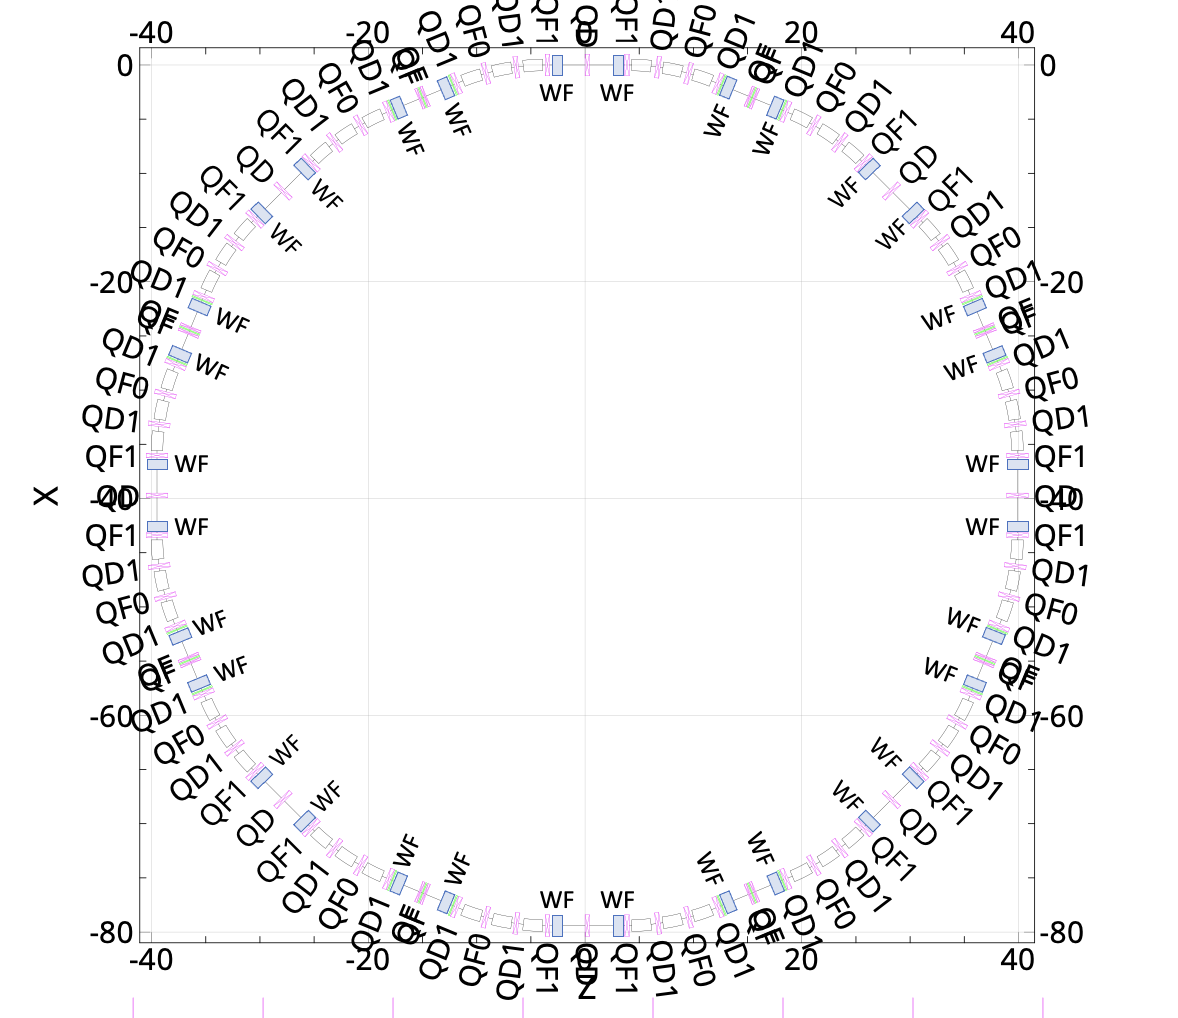
\includegraphics[width=0.9\columnwidth]{4_Nuclotron_16.png}
			\end{minipage}
		\end{column}
	\end{columns}
\end{frame}
%------------------------------------------------
\begin{frame}
	\frametitle{NICA bypass}
	\centering
	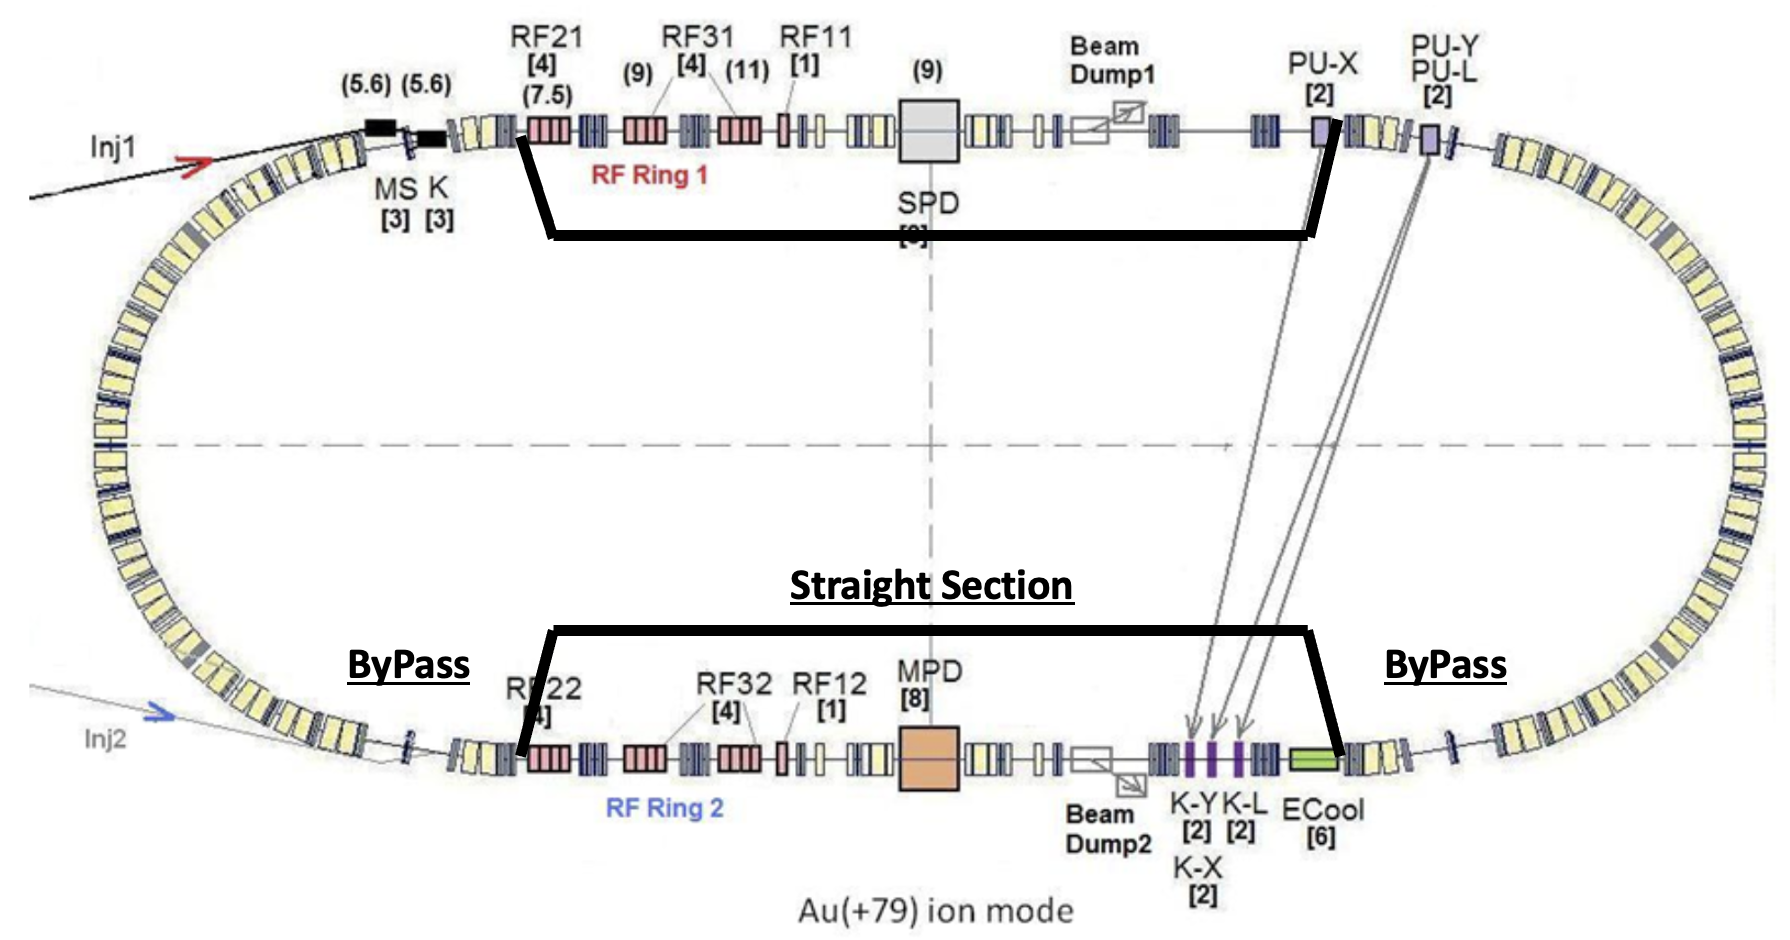
\includegraphics[width=0.65\columnwidth]{4_NICA_bypass.png}
\footnotetext[10]{Колокольчиков С.Д. и др. Проектирование Каналов Bypass в Ускорительном Комплексе NICA для Экспериментов с Поляризованными Пучками по Поиску ЭДМ. Яд. Физ. и Инж. том 15, номер 5, стр. 457-463 (2024). DOI: 10.56304/S2079562924050257}
\footnotetext[11]{S. Kolokolchikov et al. ByPass optics design in NICA storage ring for experiment with polarized beams for EDM search. J.Phys.Conf.Ser. Vol. 2687, 022026 (2024). DOI: 10.1088/1742-6596/2687/2/022026}
\end{frame}
%------------------------------------------------
\begin{frame}
	\frametitle{Декогеренция спина}
	\centering
	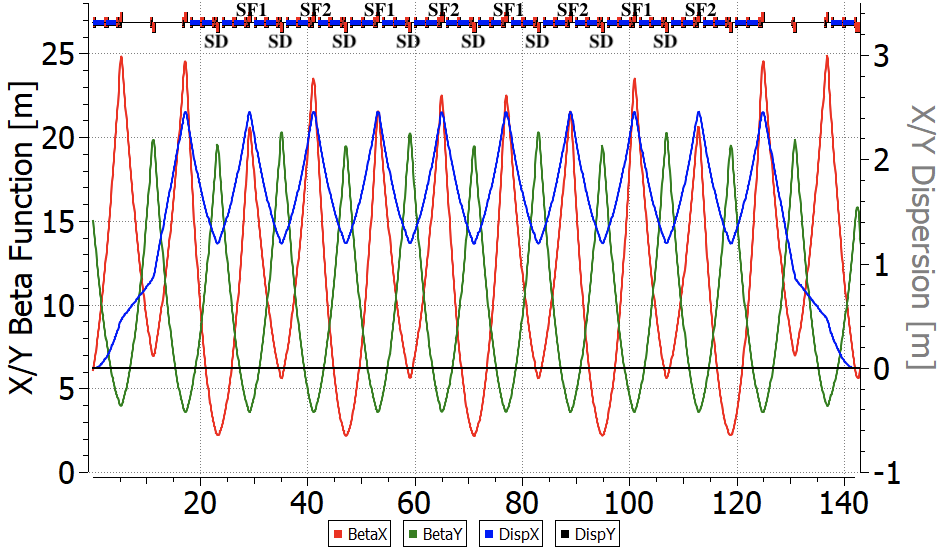
\includegraphics[width=0.55\columnwidth]{4_NICA_arc.png}
	\footnotetext[12]{Kolokolchikov S. et al. Spin Coherence and Betatron Chromaticity of Deuteron Beam in “Quasi-Frozen” Spin Regime. Phys. Atom. Nuclei 86, 2684–2688 (2023). DOI: 10.1134/S106377882311025X}
	\footnotetext[13]{S. Kolokolchikov et al. Spin coherence and betatron chromaticity of deuteron beam in NICA storage ring. J.Phys.Conf.Ser. Vol. 2687, 022027 (2024). DOI: 10.1088/1742-6596/2687/2/022027}
\end{frame}
%------------------------------------------------
\section{Результаты}
%------------------------------------------------
\begin{frame}
	\frametitle{Основные результаты работы}
	\begin{itemize}
		\item Изменение коэффициента проскальзывания в резонансной структуре повышает эффективность стохастического охлаждения, но эффекты ВПР делают предпочтительной регулярную структуру для экспериментов с тяжелыми ионами;
		\vspace{1em}
		\item Для коллайдерных экспериментов с поляризованными протонами резонансная структура повышает критическую энергию, искажая дисперсионную функцию;
		\vspace{1em}
		\item Численные исследования выявили нестабильность продольного фазового движения при прохождении критической энергии. Процедура скачка критической энергии помогает решить эту проблему. Экспериментальные данные с синхротрона У-70 согласуются с численными оценками, учитывающими высшие порядки разложения коэффициента уплотнения орбиты и импедансы для различных интенсивностей сгустка;
	\end{itemize}
\end{frame}
%------------------------------------------------
\begin{frame}
	\frametitle{Основные результаты работы}
	\begin{itemize}
		\item Скачок критической энергии ограничен его величиной и темпом изменения. Различия применения гармонического и барьерного ВЧ влияют на скачок. Оценки показывают ограничения на параметры сгустка из-за продольной микроволновой неустойчивости;
		\vspace{1em}
		\item Изучена спиновая динамика для измерения ЭДМ. Предложена концепция квази-замороженного спина с использованием метода фильтров Вина в кольце с обводными каналами;
		\vspace{1em}
		\item Модернизированный синхротрон Nuclotron сохраняет функцию бустера для коллайдера NICA. В 8/16-периодичных структурах возможны эксперименты по ЭДМ и поиск аксиона.
	\end{itemize}
\end{frame}
%------------------------------------------------
\begin{frame}
	\frametitle{Апробация работы}
	Основные результаты работы были представлены~на:
	\small
	\begin{itemize}
		\item 63, 65, 66-ая Всероссийская научная конференция МФТИ в 2020, 2023, 2024 гг. г. Долгопрудный,
		Россия;
		\item XXVII и XXVIII Всероссийская конференции по ускорителям заряженных частиц RuPAC'21, RuPAC'23. Алушта; Новосибирск, Россия.
		\item VII, VIII, IX и X Международная конференция Лазерные и Плазменные технологии ЛаПлаз'21, ЛаПлаз'22, ЛаПлаз'23, ЛаПлаз'24, ЛаПлас'25. Москва, Россия;
		\item XIII, XIV, XVI международная конференция по ускорителям заряженных частиц IPAC'22 IPAC'23, IPAC'25. Бангкок, Тайланд; Венеция, Италия; Тайпей, Тайвань;
		\item XIX Международная конференции по спиновой физике высоких энергий DSPIN'23. Дубна, Россия;
		\item XI-я Международная конференция по ядерной физике в накопительных кольцах STORI’24. Хуэйчжоу, провинция Гуандун, Китай;
	\end{itemize}
\end{frame}
%------------------------------------------------
\begin{frame}
	\frametitle{Публикации}
	Основные результаты по теме диссертации изложены в 13 печатных
	изданиях: 10 печатных работ изданы в журналах, рекомендованных
	ВАК, 10 статьей — в журналах, индексируемых международными
	базами цитирования Scopus и Web of Science.
	\small
	\begin{itemize}
		\item	1. (to be published) Kolokolchikov S.D., et al. Features of dual-purpose structure for heavy ion and light particles, Nucl.Sci. and Tech.
		\item	2. Колокольчиков С.Д., Сеничев Ю.В. Магнито-оптическая Структура Коллайдера NICA c Высокой Критической Энергией. Яд. Физ. и Инж. том 13, номер 1, стр. 27-36 (2022). DOI: 10.56304/S2079562922010171
		\item	3. Колокольчиков С.Д., Сеничев Ю.В. Особенности Прохождения и Повышения Критической Энергии Синхротрона. Яд. Физ. и Инж. том 14, номер 6, стр. 587-592 (2023).  DOI: 10.56304/S2079562923010153
		\item	4. Kolokolchikov S.D., Senichev. Y.V. \& Kalinin. V.A. Transition Energy Crossing in Harmonic RF at Proton Synchrotron U-70. Phys. Atom. Nuclei 87, 1355–1362 (2024). DOI: 10.1134/S106377882410020X
	\end{itemize}
\end{frame}
%------------------------------------------------
\begin{frame}
	\frametitle{Публикации}
	\small
	\begin{itemize}
		\item	5. Kolokolchikov S.D. et al. Transition Energy Crossing in NICA Collider of Polarized Proton Beam in Harmonic and Barrier RF. Phys. Atom. Nuclei 87, 1449–1454 (2024). DOI: 10.1134/S1063778824100211
		\item	6. Kolokolchikov S. et al. Longitudinal Dynamic in NICA Barrier Bucket RF System at Transition Energy Including Impedances in BLonD. Phys. Part. Nuclei Lett. 21, 419–424 (2024). DOI: 10.1134/S1547477124700389
		\item	7. Kolokolchikov S., Acceleration and crossing of transition energy investigation using an RF structure of the barrier bucket type in the NICA accelerator complex. J.Phys.Conf.Ser. Vol. 2420, 012001 (2023). DOI: 10.1088/1742-6596/2420/1/012001
		\item	8. Kolokolchikov S. et al. Transition Energy Crossing of Polarized Proton Beam at NICA. Phys. Atom. Nuclei 87, 212–215 (2024). DOI: 10.1134/S1063778824700054
	\end{itemize}
\end{frame}
%------------------------------------------------
\begin{frame}
	\frametitle{Публикации}
	\small
	\begin{itemize}
		\item	9. (to be published) Kolokolchikov S.D., et al. Quasi-frozen spin for both deuteron and proton beam at periodic EDM storage ring lattice, Nucl.Sci. and Tech.
		\item	10. Колокольчиков С.Д. и др. Проектирование Каналов Bypass в Ускорительном Комплексе NICA для Экспериментов с Поляризованными Пучками по Поиску ЭДМ. Яд. Физ. и Инж. том 15, номер 5, стр. 457-463 (2024). DOI: 10.56304/S2079562924050257
		\item	11. S. Kolokolchikov et al. ByPass optics design in NICA storage ring for experiment with polarized beams for EDM search. J.Phys.Conf.Ser. Vol. 2687, 022026 (2024). DOI: 10.1088/1742-6596/2687/2/022026
		\item	12. Kolokolchikov S. et al. Spin Coherence and Betatron Chromaticity of Deuteron Beam in “Quasi-Frozen” Spin Regime. Phys. Atom. Nuclei 86, 2684–2688 (2023). DOI: 10.1134/S106377882311025X
		\item	13. S. Kolokolchikov et al. Spin coherence and betatron chromaticity of deuteron beam in NICA storage ring. J.Phys.Conf.Ser. Vol. 2687, 022027 (2024). DOI: 10.1088/1742-6596/2687/2/022027
	\end{itemize}
\end{frame}
%------------------------------------------------



%------------------------------------------------
\section{Заключение}
%------------------------------------------------
\begin{frame}
	\frametitle{Благодарность}
	\begin{center}
		Спасибо за внимание!
	\end{center}
	
\end{frame}
%------------------------------------------------
\begin{frame}
	\begin{center}
		Back up
	\end{center}
\end{frame}
%------------------------------------------------
\begin{frame}
	\frametitle{Подавление дисперсии}
	\begin{figure}
		\centering
		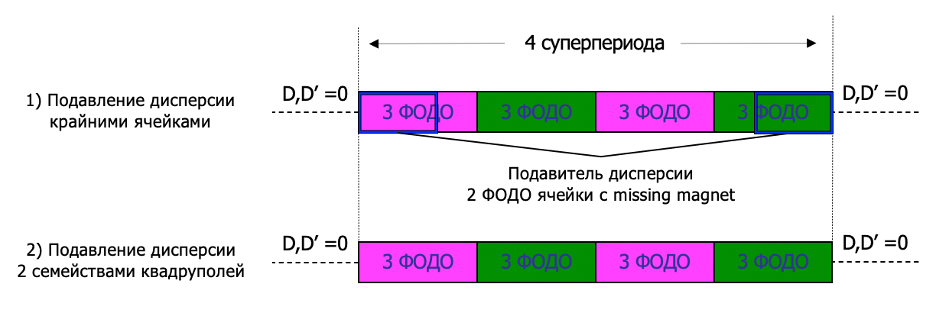
\includegraphics[width=0.8\linewidth]{images/2_disp_supp_shemes}
	\end{figure}
\end{frame}
%------------------------------------------------
\begin{frame}
	\frametitle{Критическая энергия}
	Уравнения продольного движения:
	\begin{equation}
		\begin{cases}
			\begin{aligned}
				& \dv{\tau}{t}=\eta(\delta) \cdot \frac{h \cdot \Delta E}{\beta^2 \cdot E_0} \\
				& \dv{(\Delta E)}{t}=\frac{V(\tau)}{T_0}
			\end{aligned}
		\end{cases}
		\label{eq:long_motion_eq_t}
	\end{equation}	
	Коэффициент уплотнения орбиты (momentum compaction factor):
	\begin{equation}
		\alpha_c=\frac{1}{C_0} \dv{C}{\delta}=\alpha_0+2 \alpha_1 \delta+3 \alpha_2 \delta^2+\cdots \equiv \frac{1}{\gamma_{\textrm{tr}}^2} = \frac{1}{C} \int_0^{\mathrm{C}} \frac{D(s)}{\rho(s)} d s,
		\label{eq:alpha}
	\end{equation}
	Коэффициент проскальзывания (slip-factor):
	\begin{equation}
		\eta = \eta_{0} = \alpha_{0} - \frac{1}{\gamma_{0}^2}.
		\label{eq:slip-factor_0}
	\end{equation}
\end{frame}
%------------------------------------------------
\begin{frame}
	\frametitle{Суперпериодическая модуляция}
	Уравнение для дисперсионной функции с бипериодической переменной фокусировкой
	\begin{equation}
		\dv[2]{D}{s}+\left[K(s)+\varepsilon k(s)\right]D=\frac{1}{\rho(s)} ,
		\label{eq:disp_eq}
	\end{equation}
	MCF для одного суперпериода в первом приближении
	\begin{equation}
		\begin{aligned}
			\alpha_s= & \frac{1}{\nu^2}\left\{1+\frac{1}{4(1-k S / \nu)}\left(\frac{\bar{R}}{\nu}\right)^4 \frac{g_k^2}{\left[1-(1-k S / \nu)^2\right]^2}\right\}.
		\end{aligned}
		\label{eq:alpha_gradient}
	\end{equation}
	\begin{figure}
		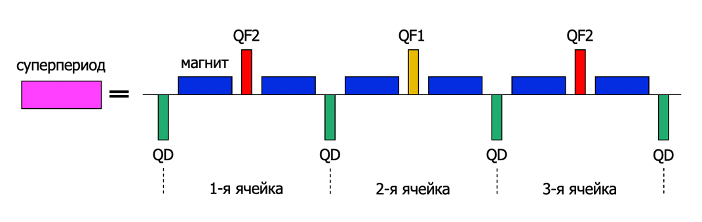
\includegraphics[width=0.6\linewidth]{images/2_superperiod}
	\end{figure}
\end{frame}
%------------------------------------------------
\begin{frame}
	\frametitle{Оптимальное время жизни пучка}
	Временная эволюция эмиттанса и разброса импульса в присутствии процессов охлаждения
	\begin{equation}
		\dv{\varepsilon}{t} =\underbrace{-\frac{1}{\tau_{\text{tr}}} \cdot \varepsilon}_{\text{cooling}}+\underbrace{\left(\dv{\varepsilon}{t}\right)_{\text{IBS}}}_{\text{heating}}, \quad
		\dv{\delta^2}{t} =\underbrace{-\frac{1}{\tau_{\text{long}}} \cdot \delta^2}_{\text{cooling}}+\underbrace{\left(\dv{\delta^2}{t}\right)_{\text{IBS}}}_{\text{heating}}.
	\end{equation}
	Для независимых от времени, стационарных значений, производные по времени становятся равными нулю
	\begin{equation}
		\varepsilon_{\textrm{st}}=\left.\tau_{\text{tr}} \cdot\left(\dv{\varepsilon}{t}\right)_{\text{IBS}}\right|_{\varepsilon=\varepsilon_{\text{st}}}, \quad
		\delta_{st}^2=\left.\tau_{\text{long}} \cdot\left(\dv{\delta^2}{t}\right)_{\text{IBS}}\right|_{\delta^2=\delta_{\text{st}}^2}.
	\end{equation}
\end{frame}
%------------------------------------------------
\begin{frame}
	\frametitle{Прохождение критической энергии}
	Характерное время \textit{адиабатичности} и \textit{нелинейность} продольного движения
	\begin{equation}
		\tau_{\textrm{ad}}=\left(\frac{\pi\beta^2mc^2\gamma_{\textrm{tr}}^4}{\dot{\gamma}\omega_0^2heV\left|\cos{\phi_{\textrm{s}}}\right|}\right)^{1/3}; \quad\quad
		\tau_{\textrm{nl}}=\frac{\eta_1\hat{\delta}}{\frac{2\dot{\gamma}}{{\gamma_{\textrm{tr}}}^3}}=\gamma_{\textrm{tr}}\frac{\frac{3}{2}\beta^2+\gamma_{\textrm{tr}}^2\alpha_1}{2\dot{\gamma}}\
	\end{equation}
	
	\begin{figure}
		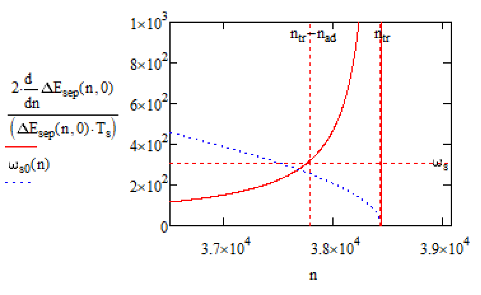
\includegraphics[width=0.4\columnwidth]{3_adiabatic_time.png}
		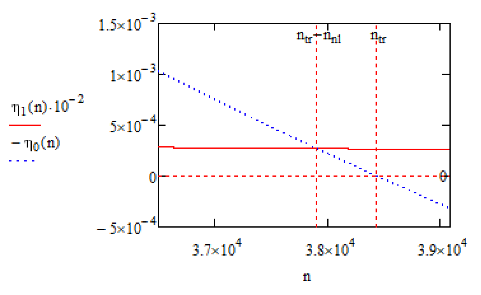
\includegraphics[width=0.4\columnwidth]{3_nonlin_time.png}
	\end{figure}
\end{frame}
%------------------------------------------------
\begin{frame}
	\frametitle{Моделирование динамики}
	\centering
	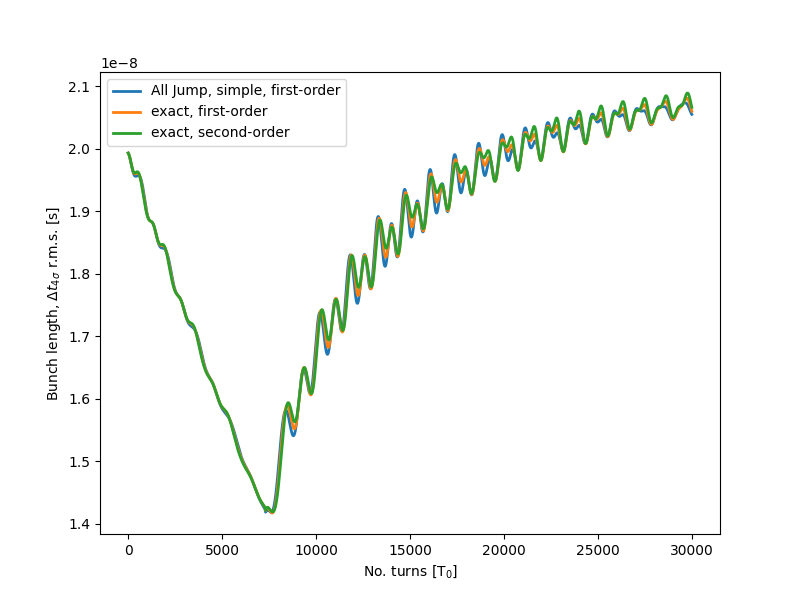
\includegraphics[width=0.275\columnwidth]{3_jump_beam_lenght.png}
	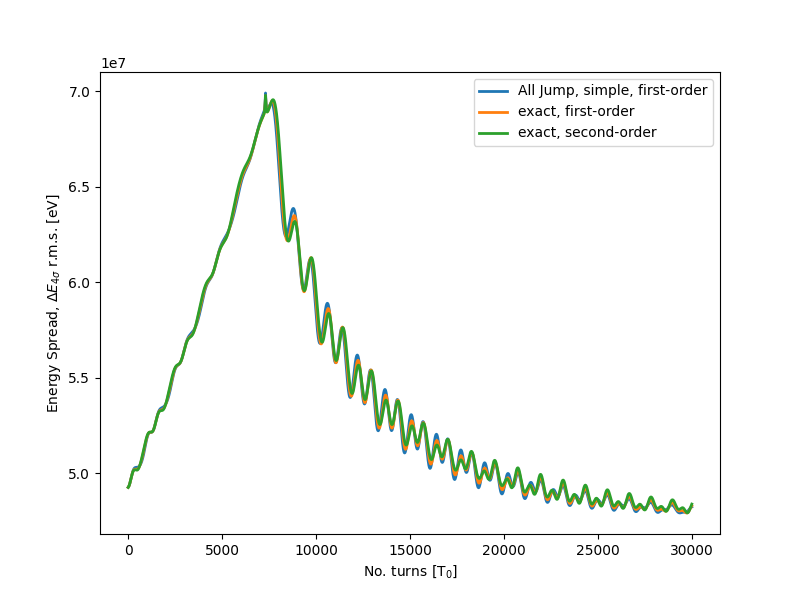
\includegraphics[width=0.275\columnwidth]{3_jump_energy_spread.png}
	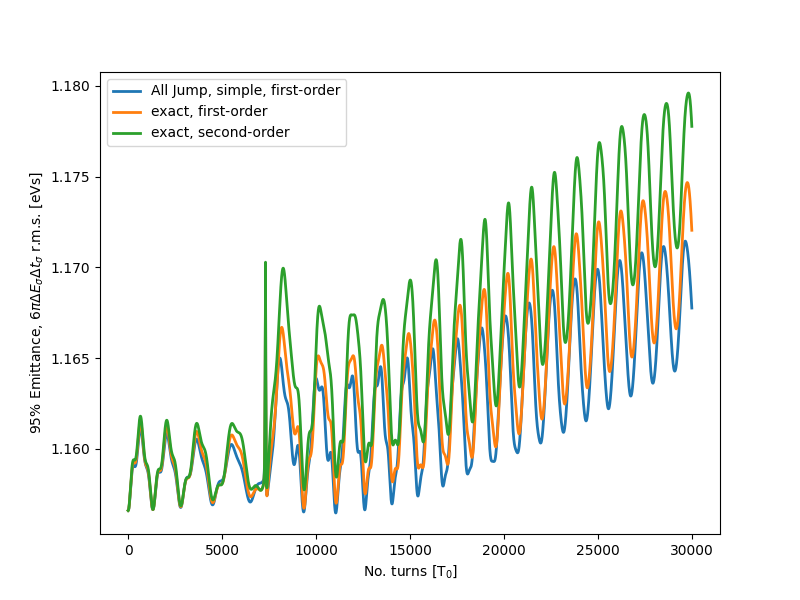
\includegraphics[width=0.275\columnwidth]{3_jump_emit.png}
	
	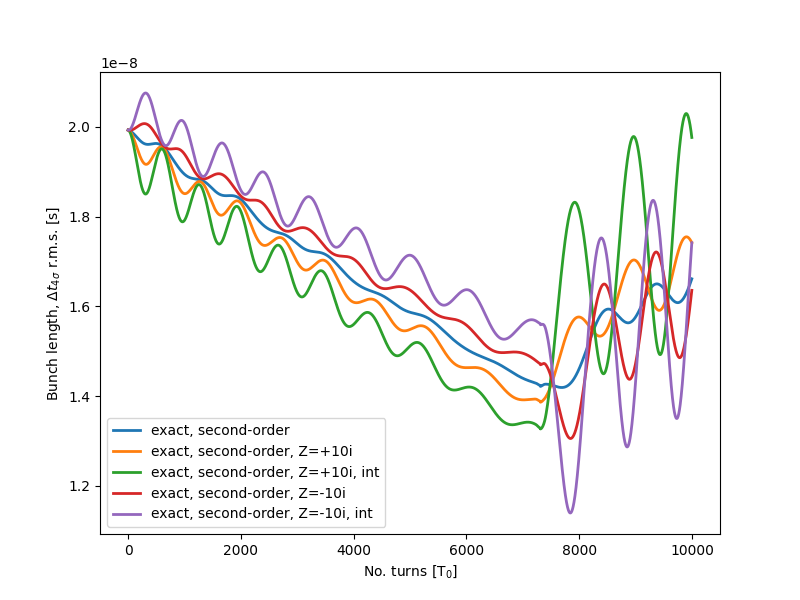
\includegraphics[width=0.275\columnwidth]{3_jump_imp_beam_lenght.png}
	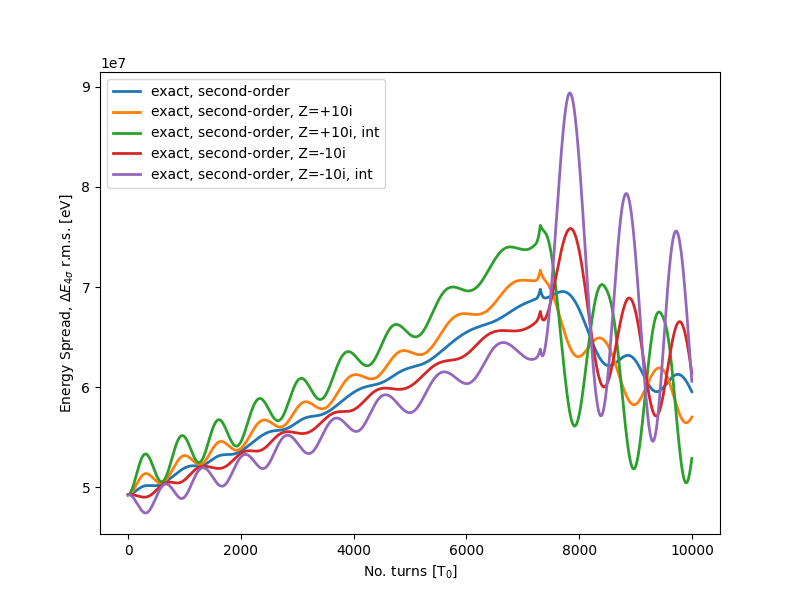
\includegraphics[width=0.275\columnwidth]{3_jump_imp_energy_spread.png}
	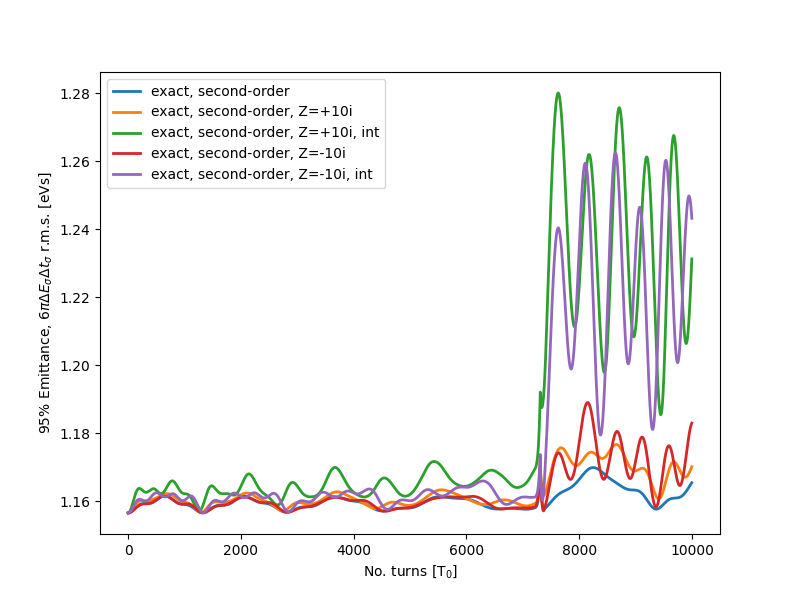
\includegraphics[width=0.275\columnwidth]{3_jump_imp_emit.png}
\end{frame}
%------------------------------------------------
\begin{frame}
	\frametitle{Скачок критической энергии в гармоническом ВЧ}
	\centering
	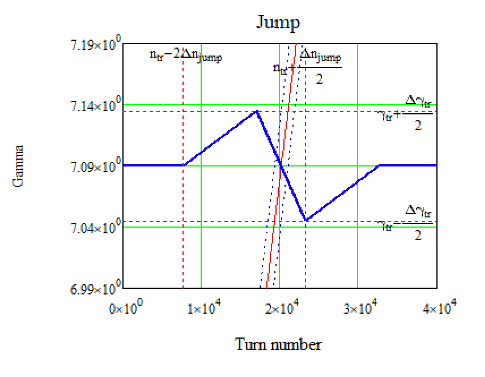
\includegraphics[width=0.4\columnwidth]{3_g_tr_harmonic.png}
	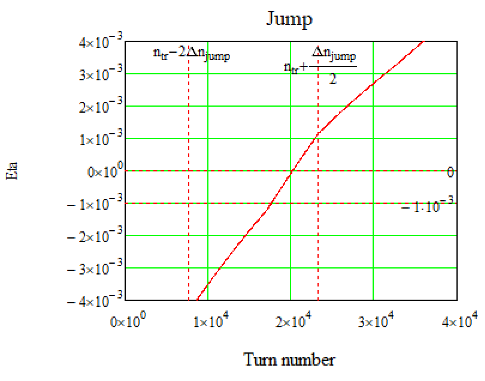
\includegraphics[width=0.4\columnwidth]{3_eta_tr_harmonic.png}
\end{frame}
%------------------------------------------------
\begin{frame}
	\frametitle{Скачок критической энергии в барьерном ВЧ I}
	\centering
	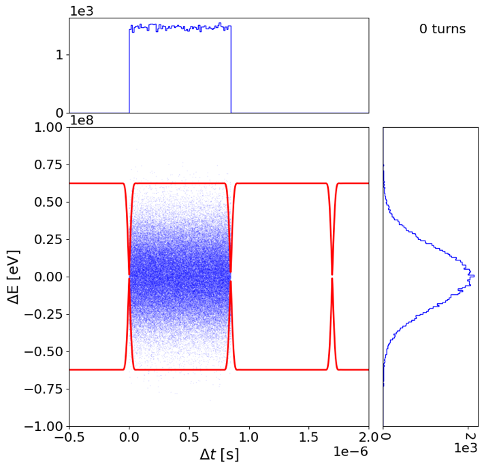
\includegraphics[width=.4\columnwidth]{3_BB_PS_near_tr}
	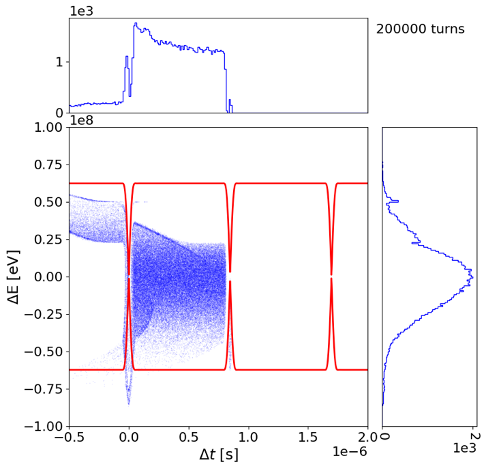
\includegraphics[width=.4\columnwidth]{3_BB_PS_near_tr_2}
\end{frame}
%------------------------------------------------
\begin{frame}
	\frametitle{Скачок критической энергии в барьерном ВЧ II}
	\centering
	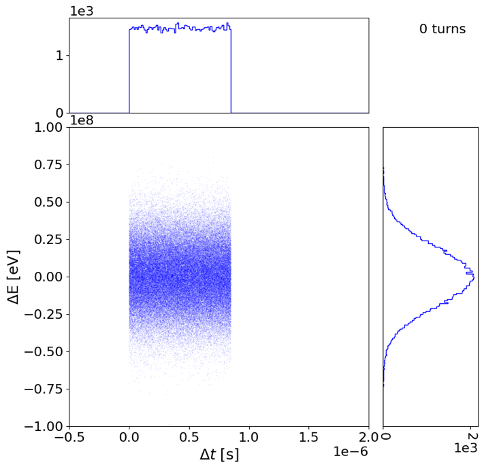
\includegraphics[width=.4\columnwidth]{3_BB_PS_jump}
	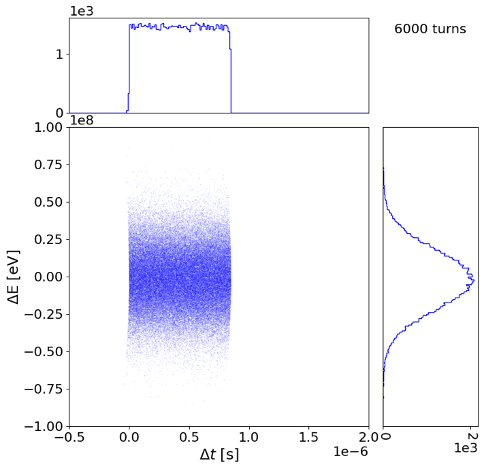
\includegraphics[width=.4\columnwidth]{3_BB_PS_jump_2}
\end{frame}
%------------------------------------------------
\begin{frame}
	\frametitle{Влияние импеданса}
	\centering
	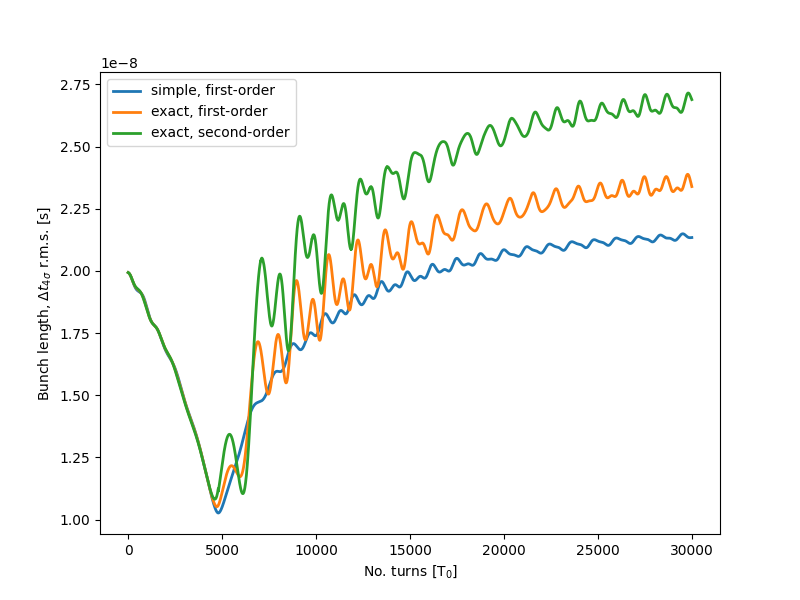
\includegraphics[width=0.275\columnwidth]{3_eta_beam_lenght.png}
	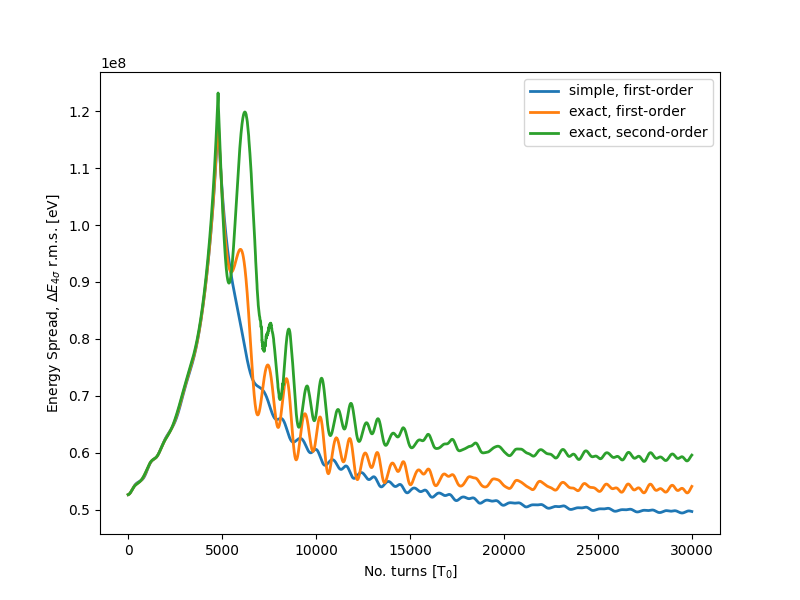
\includegraphics[width=0.275\columnwidth]{3_eta_energy_spread.png}
	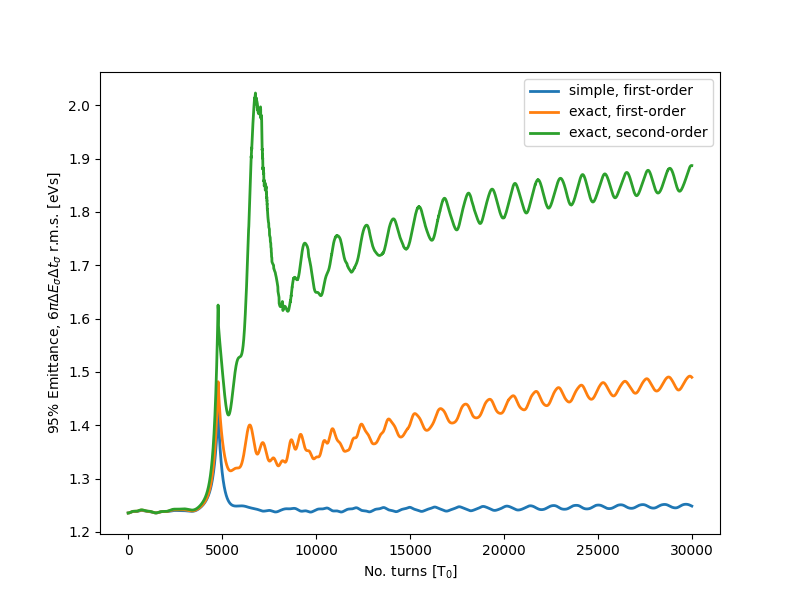
\includegraphics[width=0.275\columnwidth]{3_eta_emit.png}
	
	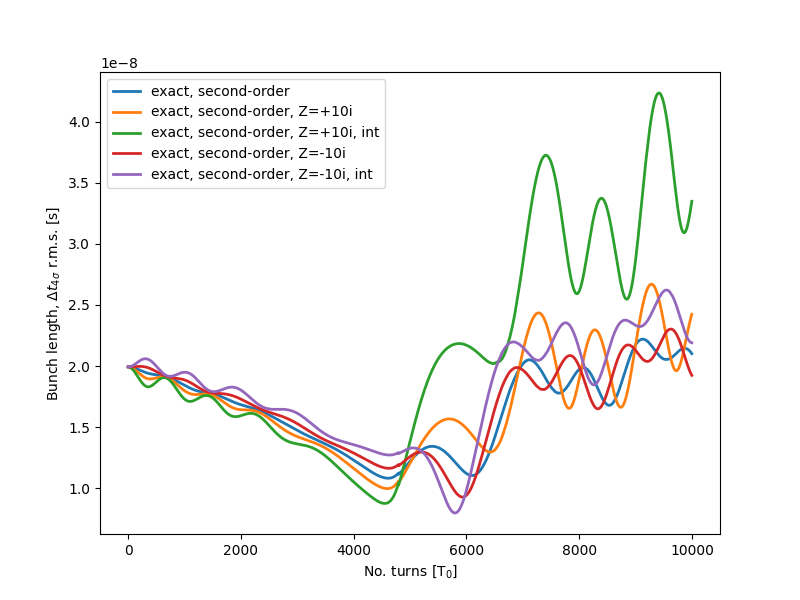
\includegraphics[width=0.275\columnwidth]{3_wo_jump_beam_lenght.png}
	\includegraphics[width=0.275\columnwidth]{3_wo_jump_energy_spread.png}
	\includegraphics[width=0.275\columnwidth]{3_wo_jump_emit.png}
\end{frame}
%------------------------------------------------
\begin{frame}
	\frametitle{Модернизация Nuclotron 8-ми периодическая структура}
	\centering
	\includegraphics[width=0.45\columnwidth]{4_Nuclotron_8_def1.png}
	\includegraphics[width=0.45\columnwidth]{4_Nuclotron_8_def2.png}
\end{frame}
%------------------------------------------------

\end{document}
